\documentclass[11pt]{article}
\usepackage[a4paper,margin=2.5cm]{geometry}
\usepackage[T1]{fontenc}
\usepackage[utf8]{inputenc}
\usepackage{amsmath,amssymb}
\usepackage{booktabs,array}
\usepackage{graphicx}
\usepackage{xcolor}
\usepackage[numbers,sort&compress]{natbib}
\usepackage[colorlinks=true,linkcolor=blue!50!black,citecolor=blue!50!black,urlcolor=blue!50!black]{hyperref}
\graphicspath{{../../examples/}}

\newcommand{\qgZ}{qg_Z}
\newcommand{\qgX}{qg_X}
\newcommand{\qgY}{qg_Y}

\title{Lo que el sesgo polar puede y no puede hacer en criptografía:\\
distinguir deriva de espionaje en BB84, y aleatoriedad cuántica certificada}
\author{Vicente Humberto Monteverde\\
\small Universidad del Museo Social Argentino (UMSA), Argentina\\
\small ORCID 0000-0001-8884-4811}
\date{\small Borrador del 30 de septiembre de 2026 (traducción de la versión en inglés)}

\renewcommand{\abstractname}{Resumen}
\renewcommand{\tablename}{Tabla}
\renewcommand{\figurename}{Figura}
\renewcommand{\refname}{Referencias}

\begin{document}
\maketitle

\begin{abstract}
Nos preguntamos dónde es útil para la criptografía la descripción qg de un qubit, $\qgZ=\langle\sigma_z\rangle$
y sus compañeros $\qgX,\qgY$~\cite{monteverde2026qang}. La criptografía post-cuántica (encapsulamiento de
claves basado en retículos, como ML-KEM~\cite{fips203}) es clásica y no tiene lugar para ella. La
criptografía cuántica sí, porque sus datos crudos son valores qg. (i) En BB84~\cite{bennett1984} sobre un
canal de qubits con relajación, la suma $A_Z=qg(0)+qg(1)$ de los sesgos polares recibidos es un testigo de
T1. La relajación natural lo aumenta, mientras que el ataque de interceptar y reenviar agrega errores
simétricos que lo dejan igual. Un monitor de razón de verosimilitud construido sobre él detecta ese ataque
tan bien como el monitor estándar de la tasa de error (QBER), pero no da falsas alarmas cuando se degrada
el T1 de la memoria, donde el monitor de QBER se dispara en el 48--100\% de las ventanas. Por
construcción no detecta a un atacante que imita a T1, al que el monitor de QBER sí detecta: los dos son
complementarios y ninguno cambia la tasa de clave secreta. Con claves finitas~\cite{tomamichel2012} el
diagnóstico sale gratis del bloque ya corregido: con $10^5$ bits de clave atribuye bien cada bloque,
incluido un ataque pequeño escondido bajo la deriva. (ii) Para un generador de números aleatorios de un
qubit con medición confiable, la min-entropía certificada es
$H_{\min}(Z|E)=-\log_2\big[(1+\sqrt{1-\qgX^2-\qgY^2})/2\big]$, independiente de $\qgZ$. La estimación
habitual a partir del sesgo de la salida es insegura siempre que el estado sea mixto: certifica 0.97 bits
por disparo donde solo 0.015 son privados. Una estimación qg a partir de rondas de prueba con rotaciones
$\pm$ es segura en todas las corridas, y una calibración de la lectura recupera un 10--50\% más de bits
certificados. En modelos de ruido de iones atrapados de IonQ, con un ion del entorno que aprende la
salida, la estimación ingenua se queda cerca de 1 bit mientras que la estimación qg sigue siendo segura y
captura el 82--90\% de la aleatoriedad privada. Todos los resultados son simulaciones, reproducidas por
scripts y fijadas por tests de regresión.
\end{abstract}

\section{Dónde qg no se aplica: criptografía post-cuántica}

Los esquemas post-cuánticos como ML-KEM (Kyber)~\cite{fips203} o las firmas basadas en retículos y en
funciones hash corren en computadoras clásicas y están diseñados para resistir ataques cuánticos. No
involucran qubits ni estadísticas de medición, así que una coordenada para mediciones de qubits no tiene
nada que aportar. La amenaza que responden, el algoritmo de Shor, tampoco se beneficia de qg; el notebook
de referencia del proyecto lo documenta como una no-aplicación. Lo decimos primero para que el resto no se
lea como una afirmación sobre seguridad post-cuántica.

\section{BB84: ¿deriva o espía?}\label{sec:bb84}

\paragraph{Escenario.} Alice envía $|0\rangle,|1\rangle$ (base Z) o $|\pm\rangle$ (base X); el qubit espera
en una memoria o canal con amortiguamiento de amplitud $\gamma$ (T1) y desfase $p$; Bob mide con un
detector asimétrico ($e_{01}=0.005$, $e_{10}=0.01$). Esto corresponde a enlaces entre qubits materiales y
a demostraciones en chip, no a enlaces de polarización de fotones, cuyo ruido es mayormente unital. Cada
estado enviado da un valor qg en Bob,
\begin{equation}
qg(0)=1-2e(0\!\to\!1),\quad qg(1)=-1+2e(1\!\to\!0),\quad
A_Z=qg(0)+qg(1)=2\,[e(1\!\to\!0)-e(0\!\to\!1)],
\end{equation}
y lo mismo en X. $A_Z$ es el testigo de T1 del promedio del registro del trabajo
complementario~\cite{monteverde2026witness}: la relajación crea solo errores $1\to0$ y lo aumenta, mientras
que interceptar y reenviar una fracción $f$ de los qubits agrega errores $f/4$ en cada categoría y lo deja
igual. El canal de referencia tiene $\gamma_0=0.02$, $p_0=0.01$.

\paragraph{Monitores.} Ventanas de $N$ bits comparados, con 1\% de falsas alarmas sobre la referencia. El
\emph{monitor de QBER} prueba el conteo total de errores. El \emph{monitor qg} es una razón de
verosimilitud generalizada sobre los cuatro conteos de error, en la que ``ataque'' ($f>0$) debe superar
tanto a ``referencia'' como a ``deriva de T1'' ($\gamma$ libre).

\begin{table}[t]
\centering\small
\caption{Tasas de alarma (1000 ventanas de $N=2000$ bits comparados). La última columna es la fracción
secreta de Shor--Preskill $1-h(Q_Z)-h(Q_X)$~\cite{shorpreskill2000}.}
\label{tab:bb84}
\begin{tabular}{lccc}
\toprule
escenario & monitor QBER & monitor qg & fracción secreta\\
\midrule
referencia & 0.007 & 0.006 & 0.720\\
deriva de T1, $\gamma$ $0.02\to0.04$ & 0.478 & \textbf{0.009} & 0.640\\
deriva de T1, $\gamma$ $0.02\to0.06$ & 0.962 & \textbf{0.006} & 0.567\\
interceptar y reenviar, $f=0.02$ & 0.218 & 0.271 & 0.668\\
interceptar y reenviar, $f=0.05$ & 0.861 & 0.823 & 0.594\\
interceptar y reenviar, $f=0.10$ & 1.000 & 0.994 & 0.481\\
ataque que imita a T1 ($\gamma$ extra $=0.04$) & \textbf{0.962} & 0.006 & 0.567\\
\bottomrule
\end{tabular}
\end{table}

\begin{figure}[t]
\centering
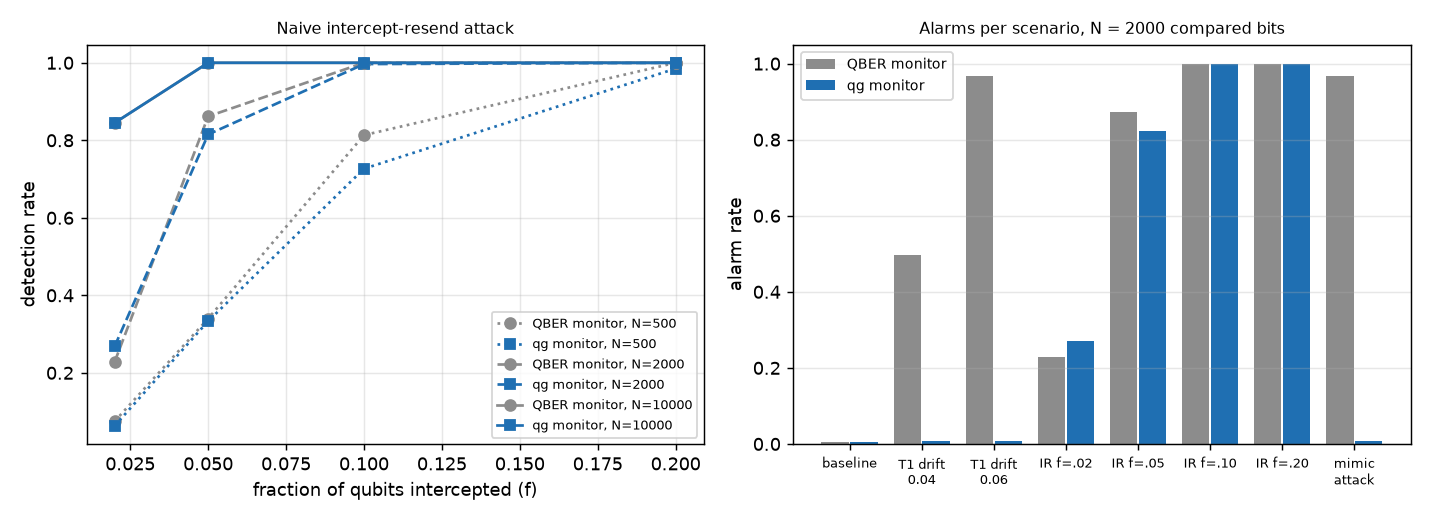
\includegraphics[width=\linewidth]{bb84_qg_eve_vs_noise.png}
\caption{Izquierda: detección de interceptar y reenviar según la fracción interceptada, para $N=500$, 2000
y 10{,}000 bits comparados. Derecha: tasas de alarma por escenario con $N=2000$.}
\label{fig:bb84}
\end{figure}

\paragraph{Resultados} (Tabla~\ref{tab:bb84}, Fig.~\ref{fig:bb84}).
\begin{itemize}
\item \emph{Igual detección, menos falsas alarmas.} El monitor qg detecta interceptar y reenviar tan bien
como el monitor de QBER para todo $N$ y $f$, pero se queda callado cuando T1 se degrada. El monitor de
QBER se dispara en el 48--100\% de esas ventanas.
\item \emph{El precio, por diseño.} Una atacante que acopla el qubit a su ancilla mediante una interacción
de amortiguamiento de amplitud es, desde el lado de Bob, idéntica a una deriva de T1. El monitor qg no la
ve y el de QBER sí. Usados juntos, QBER dice que algo cambió y qg dice qué tipo de cambio es.
\item \emph{Sin ganancia de seguridad.} La fracción secreta cae igual en todos los casos. Una prueba de
seguridad debe atribuir cada error a Eve~\cite{scarani2009}. El monitor qg es un diagnóstico operativo.
\end{itemize}

\section{BB84 con claves finitas}\label{sec:finite}

Los enlaces reales destilan claves a partir de bloques finitos. Usamos la cota de Tomamichel \emph{et
al.}~\cite{tomamichel2012} sobre el canal de la Sec.~\ref{sec:bb84}: $n$ bits de clave en Z, $k$ bits de
prueba en X, se aborta si el error de prueba supera $Q_{\rm tol}$, y
\begin{equation}
\ell=n\big[1-h(Q_{\rm tol}+\mu)\big]-1.1\,n\,h(Q_Z)-\log_2\frac{2}{\varepsilon_{\rm sec}^2\varepsilon_{\rm cor}},\qquad
\mu=\sqrt{\frac{n+k}{nk}\,\frac{k+1}{k}\,\ln\frac{2}{\varepsilon_{\rm sec}}},
\end{equation}
con $\varepsilon_{\rm sec}=\varepsilon_{\rm cor}=5\times10^{-11}$, $M=(\sqrt n+\sqrt k)^2$ señales y tasa
$(1-\varepsilon_{\rm rob})\ell/M$, donde $k$ y $Q_{\rm tol}$ se optimizan para cada $n$. Sobre la referencia,
$10^4$, $10^5$, $10^6$ y $10^7$ bits de clave conservan el 17\%, 38\%, 58\% y 73\% de la tasa asintótica de
0.707 bits por señal, y no hay clave por debajo de unos $1.2\times10^3$ bits (Fig.~\ref{fig:finite},
izquierda). La deriva y el ataque cuestan clave por igual.

\paragraph{El diagnóstico es gratis.} Después de la corrección de errores y su verificación, Bob conoce
los bits de clave de Alice. Tiene entonces los cuatro conteos de error, que son los cuatro valores qg de la
Sec.~\ref{sec:bb84}, sobre los $n$ bits de clave, sin revelar nada; anunciar una alarma cuesta a lo sumo
un bit. Los bits de un bloque abortado se descartan de todos modos, así que pueden revelarse. Usamos dos
razones de verosimilitud anidadas sobre el modelo conjunto (T1 $\gamma$ e interceptar y reenviar $f$,
ambos libres). La razón \emph{tipo ataque} prueba si hay error simétrico más allá de cualquier T1; la razón
\emph{tipo deriva} prueba si hay T1 más allá de la referencia, sea cual sea el ataque. Cada una se calibra
a 1\% de falsas alarmas sobre la referencia.

\begin{table}[t]
\centering\small
\caption{Protocolo ajustado sobre la referencia con $n=10^5$ ($k=7609$, $Q_{\rm tol}=2.67\%$): fracción de
400 bloques que abortan y que levantan cada bandera qg.}
\label{tab:finite}
\begin{tabular}{lccc}
\toprule
escenario & abortos & tipo ataque & tipo deriva\\
\midrule
referencia & 0.010 & 0.020 & 0.015\\
deriva de T1 $\gamma=0.03$ & 0.100 & 0.005 & \textbf{1.000}\\
deriva de T1 $\gamma=0.04$ & 0.557 & 0.005 & \textbf{1.000}\\
deriva de T1 $\gamma=0.06$ & 0.995 & 0.007 & \textbf{1.000}\\
interceptar y reenviar $f=0.02$ & 0.495 & \textbf{1.000} & 0.043\\
interceptar y reenviar $f=0.05$ & 1.000 & \textbf{1.000} & 0.040\\
deriva 0.04 + intercepción 0.02 & 0.995 & \textbf{1.000} & \textbf{1.000}\\
ataque que imita a T1 & 0.995 & 0.013 & 1.000\\
\bottomrule
\end{tabular}
\end{table}

\begin{figure}[t]
\centering
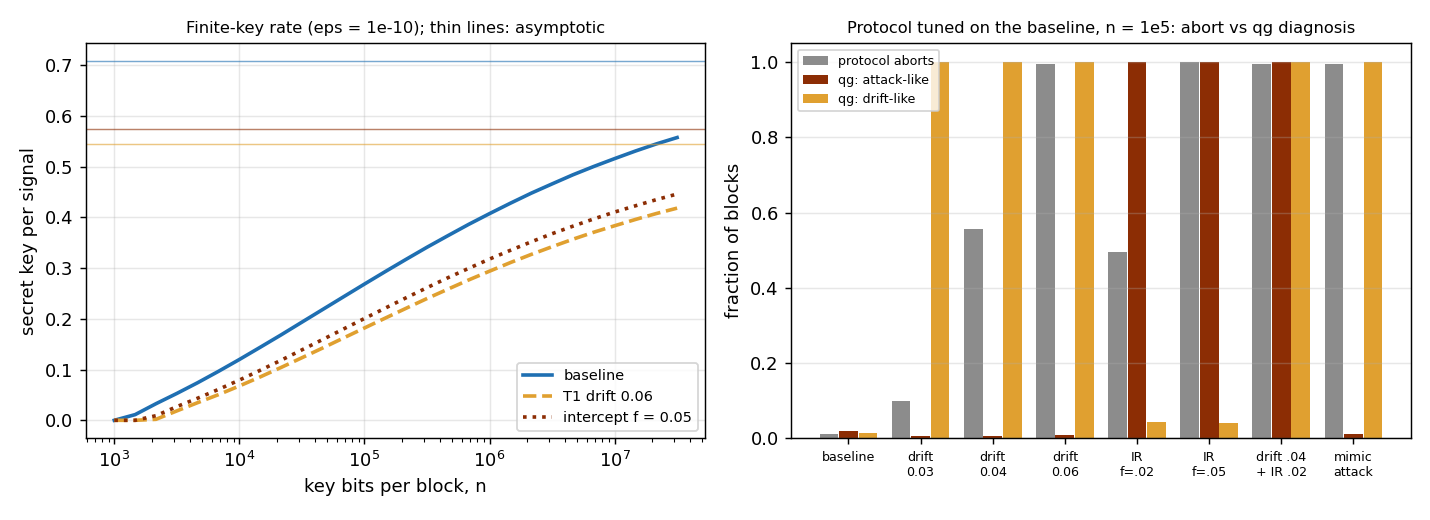
\includegraphics[width=\linewidth]{bb84_finite_key_qg.png}
\caption{Izquierda: tasa de clave finita según el tamaño del bloque (líneas finas: asintótica). Derecha:
abortos y banderas qg para un protocolo ajustado sobre la referencia con $n=10^5$.}
\label{fig:finite}
\end{figure}

\paragraph{Resultados} (Tabla~\ref{tab:finite}).
\begin{itemize}
\item \emph{Un aborto no dice por qué; las banderas qg sí.} Todo bloque con deriva, abortado o no, se marca
como deriva y no como ataque. Todo bloque con interceptar y reenviar se marca como ataque, incluida la
mitad que no abortó. Con $n=10^4$ las banderas ya están en 0.97--1.00 (0.81 para $\gamma=0.03$).
\item \emph{Un ataque escondido bajo la deriva se detecta.} Interceptar y reenviar con $f=0.02$ sobre una
memoria con deriva levanta las dos banderas en todos los bloques. El monitor de un parámetro de la
Sec.~\ref{sec:bb84} no lo ve (0.5\% de banderas de ataque).
\item \emph{Alerta temprana.} Con $\gamma=0.03$ solo aborta el 10\% de los bloques, pero la bandera de
deriva está levantada en todos. Una tendencia de $Q_Z$ también avisaría; lo que agrega qg es la
atribución.
\end{itemize}

\paragraph{Más allá de interceptar y reenviar.} Desde el lado de Bob, cualquier ataque individual es un
canal de Pauli $(p_x,p_y,p_z)$, con errores en la base Z por $p_x+p_y$ y en la base X por $p_z+p_y$. El
clonador óptimo covariante en fase con perturbación $D$, que es $(0,D,0)$, da por lo tanto exactamente los
conteos de interceptar y reenviar con $f=4D$, y se marca como ataque en todos los bloques. Una intercepción
solo en Z, $(0,0,f/2)$, da exactamente los conteos de un desfase extra (deriva de T2). El modelo de dos
familias de arriba no tenía familia de desfase, así que la deriva de T2 daba falsas alarmas de ataque en el
7.5--27\% de los bloques. Agregando esa familia, la deriva de T2 se marca como tipo T2 y las falsas
alarmas bajan al 0.7--2\%. La intercepción solo en Z se esconde entonces como deriva de T2: es un segundo
punto ciego, gemelo del ataque que imita a T1.

\paragraph{En un modelo de ruido de iones atrapados.} Reconstruimos todo el protocolo como circuitos en el
simulador en la nube de IonQ con los modelos de ruido aria-1 y forte-1. La memoria es un amortiguamiento
de amplitud hecho con una ancilla, ${\rm CRY}(2\arcsin\sqrt\gamma)$ seguido de un CX de vuelta, con
$\gamma_0=0.02$ sana y 0.03--0.06 con deriva. Eve mide y reenvía mediante una ancilla que no se lee (CX, o
H--CX--H). Hay 16 bloques de $n=k=4000$ bits por escenario y modelo. El dispositivo agrega un error casi
simétrico de 2.3--3.1\% por bit, así que el modelo de banderas incorpora dos tasas de inversión ajustadas,
$\varepsilon_Z$ y $\varepsilon_X$, y un $\gamma_0$ ajustado, todos ajustados dejando uno afuera sobre bloques
de referencia.

La atribución se traslada (Tabla~\ref{tab:ionqbb84}). Una memoria con deriva se confunde con un ataque en
a lo sumo 1 de 48 bloques, y un ataque con deriva en a lo sumo 1 de 16. La deriva 0.06 y $f=0.10$ se
atribuyen en todos los bloques. Con este tamaño de bloque y este nivel de ruido, los cambios pequeños se
marcan solo en parte. El modelo ajustado predice qué bandera sube, y la mayoría de las tasas dentro de la
dispersión de 16 bloques. Extrapolado a $n=10^5$ bits de clave, atribuye todos los escenarios en el
99--100\% de los bloques.

\begin{table}[t]
\centering\small
\caption{Circuitos BB84 en modelos de ruido de IonQ, $n=k=4000$ por bloque, 16 bloques: fracción de bloques
que levantan las banderas tipo ataque / tipo deriva, observada (predicha por el modelo ajustado).}
\label{tab:ionqbb84}
\begin{tabular}{lcc}
\toprule
escenario & aria-1 & forte-1\\
\midrule
referencia & 0.00 / 0.00 & 0.06 / 0.06\\
deriva 0.04 & 0.00 / 0.81 (0.73) & 0.00 / 0.38 (0.46)\\
deriva 0.06 & 0.00 / \textbf{1.00} & 0.00 / \textbf{1.00}\\
intercepción $f=0.05$ & \textbf{0.88} (0.96) / 0.00 & \textbf{0.81} (0.88) / 0.06\\
intercepción $f=0.10$ & \textbf{1.00} / 0.00 & \textbf{1.00} / 0.06\\
deriva 0.04 + $f=0.05$ & 0.81 / 0.81 & 0.75 / 0.31\\
\bottomrule
\end{tabular}
\end{table}

\section{Números aleatorios certificados}\label{sec:qrng}

Un generador cuántico de números aleatorios de un qubit~\cite{herrero2017} prepara $|+\rangle$ y mide Z. El
desfase y la población térmica dejan la salida sin sesgo, pero entonces parte de la aleatoriedad es ruido
clásico que un adversario que controla el entorno puede conocer. Con una medición confiable y un adversario
que tiene la purificación, sus dos estados condicionales son puros, con solapamiento
$|\rho_{01}|=r_\perp/2$. Por Helstrom~\cite{helstrom1976} y el significado operativo de la
min-entropía~\cite{konig2009},
\begin{equation}\label{eq:hmin}
P_{\rm guess}(Z|E)=\frac{1+\sqrt{1-r_\perp^2}}{2},\qquad
H_{\min}(Z|E)=-\log_2P_{\rm guess},\qquad r_\perp=\sqrt{\qgX^2+\qgY^2}.
\end{equation}
El resultado es independiente de $\qgZ$: solo la coherencia en la base medida es privada. Para un estado
puro se reduce a la expresión clásica $-\log_2\max(p_0,p_1)$. Verificamos la Ec.~\eqref{eq:hmin} contra
una purificación explícita.

\paragraph{Estimadores.} A partir de $10^4$ rondas de prueba por configuración, con la lectura
$\qgZ^{\rm meas}=a+b\,\qgZ$ ($e_{01}=0.015$, $e_{10}=0.04$) calibrada con el barrido heraldo del trabajo
complementario. Comparamos cuatro estimaciones. La \emph{ingenua} es la estimación por sesgo de la salida,
$-\log_2\max(\hat p_0,\hat p_1)$. La \emph{qg de un lado} toma $r_\perp$ de rondas de prueba en X e Y con
una sola rotación cada una. La \emph{qg $\pm$} mide cada eje con las dos rotaciones, así que el
desplazamiento $a$ se cancela. La \emph{qg calibrada} es la $\pm$ dividida por el $b$ calibrado. Todas las
estimaciones qg usan una cota inferior de $3\sigma$ sobre $r_\perp$.

\begin{table}[t]
\centering\small
\caption{Bits certificados por disparo: estimación media y, entre paréntesis, la fracción de corridas por
encima del valor real (inseguras). 300 repeticiones.}
\label{tab:qrng}
\begin{tabular}{lcccc}
\toprule
escenario & real & ingenua & qg $\pm$ & qg calibrada\\
\midrule
$|+\rangle$ ideal & 1.000 & 0.965 (0) & 0.512 (0) & 0.681 (0)\\
T2, $V=0.8$ & 0.322 & 0.964 (\textbf{1.00}) & 0.245 (0) & \textbf{0.286} (0)\\
T2, $V=0.5$ & 0.100 & 0.965 (\textbf{1.00}) & 0.077 (0) & \textbf{0.087} (0)\\
T2, $V=0.2$ & 0.015 & 0.965 (\textbf{1.00}) & 0.009 (0) & \textbf{0.010} (0)\\
térmico $p=0.05$, $V=0.9$ & 0.334 & 0.965 (\textbf{1.00}) & 0.254 (0) & \textbf{0.297} (0)\\
$e_{10}=0.10$, $V=0.95$ & 0.608 & 0.876 (\textbf{1.00}) & 0.341 (0) & \textbf{0.513} (0)\\
\bottomrule
\end{tabular}
\end{table}

\begin{figure}[t]
\centering
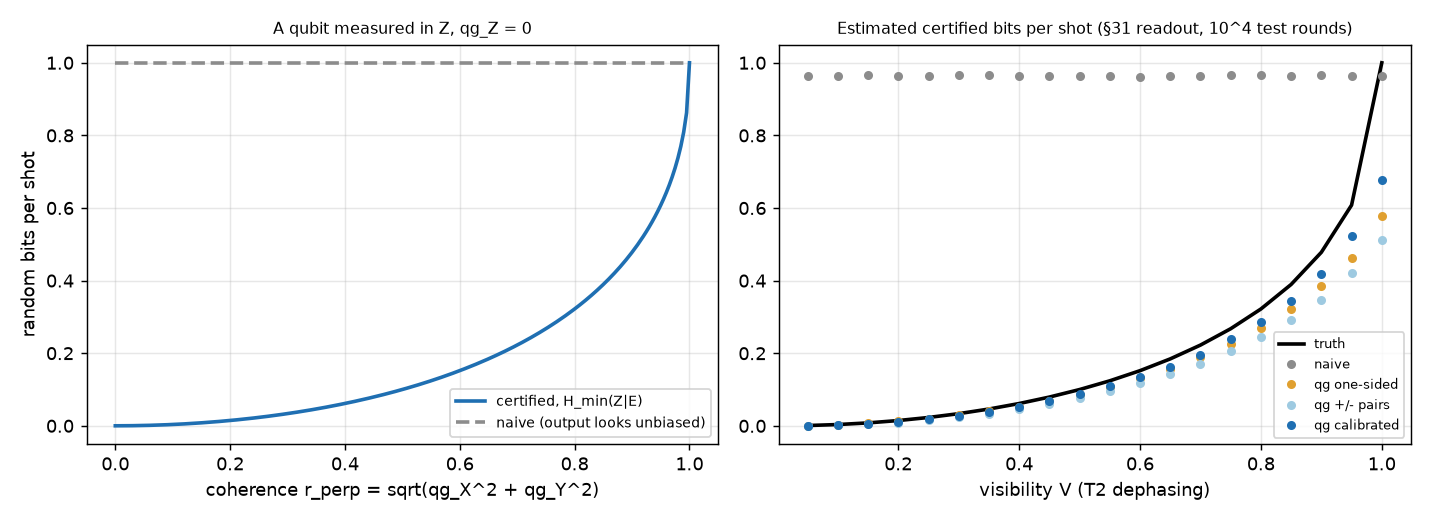
\includegraphics[width=\linewidth]{qrng_qg_certified.png}
\caption{Izquierda: bits certificados por disparo según la coherencia $r_\perp$ con $\qgZ=0$, frente a la
lectura ingenua. Derecha: estimaciones según la visibilidad $V$.}
\label{fig:qrng}
\end{figure}

\paragraph{Resultados} (Tabla~\ref{tab:qrng}, Fig.~\ref{fig:qrng}).
\begin{itemize}
\item \emph{La estimación por sesgo de la salida es insegura} siempre que el estado sea mixto: sobreestima en
todas las corridas.
\item \emph{La estimación qg es segura en todas las corridas} cuando cada eje se mide con las dos
rotaciones. Con una sola rotación, el desplazamiento de la lectura infla $r_\perp$, y con $V=0.2$ la
estimación supera el valor real en el 7\% de las corridas.
\item \emph{La calibración rinde.} Dividir por el $b$ calibrado recupera un 10--50\% más de bits
certificados.
\item \emph{Certificar una fuente casi perfecta requiere muchos disparos.} $H_{\min}$ tiene pendiente
infinita en $r_\perp=1$, el polo de qg, así que la cota de $3\sigma$ da 0.68, 0.81 y 0.89 bits por disparo
con $10^4$, $10^5$ y $10^6$ rondas de prueba.
\end{itemize}

\paragraph{En un modelo de ruido de iones atrapados.} Corrimos el certificador en el simulador en la nube de
IonQ con los modelos de ruido aria-1 y forte-1 (gratis; nada se envió a una QPU), con una fuga que el
adversario tiene realmente. Un ion fuente empieza en $|0\rangle$ y se lee en X; un segundo ion, el entorno,
aprende el valor de X mediante una compuerta de M{\o}lmer--S{\o}rensen parcial $\mathrm{MS}(0,0,\theta)$. La
salida sigue siendo una moneda justa, mientras que $H_{\min}(X|E)$ cae como en la Ec.~\eqref{eq:hmin} con
$r=|\cos2\pi\theta|$ (X y Z intercambiados). Todos los circuitos usan compuertas nativas, así que el
servicio no puede fusionar rotaciones; cada configuración tiene $10^4$ muestras, tres repeticiones por
modelo (Tabla~\ref{tab:qrngionq}). La estimación ingenua se queda en 0.97--1.00 bits y sobreestima en todas
las corridas con fuga (cuatro veces el valor real con $\theta=0.12$). La estimación qg $\pm$ es segura en
las 24 celdas y captura el 82--90\% del valor real con fuga. La lectura del simulador es casi perfecta
($b\ge0.9998$), así que la calibración no agrega nada ahí: la ganancia de la Tabla~\ref{tab:qrng} necesita
errores de lectura como los del hardware y queda por comprobarse en un dispositivo. El $r$ medido queda un
1--1.5\% por debajo del ideal, que es el error de la compuerta MS, contado correctamente como privacidad
perdida.

\begin{table}[t]
\centering\small
\caption{Bits certificados por disparo en modelos de ruido de IonQ (media de 3 corridas; aria-1 / forte-1
donde difieren). Ninguna estimación qg supera el valor real en ninguna corrida.}
\label{tab:qrngionq}
\begin{tabular}{lcccc}
\toprule
$\theta$ (vueltas) & real & ingenua & qg de un lado & qg $\pm$\\
\midrule
0 (sin fuga) & 1.000 & 0.98 & 0.69 & 0.73\\
0.04 & 0.680 & 0.99 (\textbf{insegura}) & 0.53 & \textbf{0.56 / 0.55}\\
0.08 & 0.433 & 0.98 / 0.97 (\textbf{insegura}) & 0.37 / 0.36 & \textbf{0.38 / 0.37}\\
0.12 & 0.248 & 0.99 (\textbf{insegura}) & 0.22 / 0.21 & \textbf{0.22}\\
\bottomrule
\end{tabular}
\end{table}

\section{Limitaciones}

(i) Todo es simulación: modelos de un qubit con rondas i.i.d., y modelos de ruido del proveedor en el
simulador de IonQ, no hardware. (ii) El generador de números aleatorios depende del dispositivo (medición
confiable), no es independiente del dispositivo. (iii) La Ec.~\eqref{eq:hmin} y las cotas de seguridad de
BB84, asintóticas y de clave finita, son resultados estándar; qg las escribe en cantidades medidas.
(iv) El monitor de BB84 es un diagnóstico: un atacante que imita la relajación es invisible para él, y la
tasa de clave no cambia. (v) El escenario de BB84 necesita un mecanismo de relajación (qubits materiales);
no describe enlaces de polarización de fotones. (vi) El diagnóstico con claves finitas modela solo dos
familias de error (T1 e interceptar y reenviar); otros ataques pueden quedar fuera de ambas banderas.
(vii) Las corridas en IonQ usan los modelos de ruido del proveedor en un simulador, y la memoria y el ataque
son circuitos diseñados.

\section{Disponibilidad del código}
\sloppy
\texttt{examples/bb84\_qg\_eve\_vs\_noise.py}, \texttt{examples/bb84\_finite\_key\_qg.py},
\texttt{examples/ionq\_sim\_bb84.py}, \texttt{examples/bb84\_attacks\_beyond\_ir\_qg.py},
\texttt{examples/qrng\_qg\_certified.py} y \texttt{examples/ionq\_sim\_qrng.py} en
\url{https://github.com/Viny2030/qang} (licencia MIT), con tests de regresión. Las secciones 40--44 y 49 de
\texttt{RESEARCH\_NOTES.md} dan más detalle, y \texttt{notebooks/qang\_criptografia\_colab.ipynb} reproduce
versiones rápidas en Colab.

\section*{Agradecimientos y uso de herramientas de IA}
Herramientas de IA generativa (Anthropic Claude Opus 5.5) asistieron con el código, los experimentos
numéricos, los tests y la redacción. El autor planteó las preguntas, tomó las decisiones de diseño, y
revisó y validó todo el material asistido por IA, incluido cada número informado aquí.

\bibliographystyle{unsrtnat}
\bibliography{../refs}
\end{document}
